\documentclass{report}

\usepackage[utf8]{inputenc}

\usepackage{epigraph}
\usepackage{xspace}
\usepackage{graphicx}
\usepackage{wrapfig}
\usepackage{listings}
\usepackage{verbatim}
\usepackage{multicol}
\usepackage[hmargin=3cm,vmargin=3cm]{geometry}

\newcommand{\up}[1]{\textsuperscript{#1}}
\newcommand{\imp}[1]{\text{#1}}
\renewcommand{\tt}[1]{\texttt{{{#1}}}}

\newcommand{\bcol}[1]{\begin{multicols}{2}[#1]}
\newcommand{\ecol}[0]{\end{multicols}}
\title{Design of the resource manager, or a way to dynamically start and stop
  CPU on a \textsc{Linux}-SMP system}

\author{Quentin Casasnovas}

\begin{document}

\maketitle

\newpage
\strut
\newpage

\tableofcontents


\abstract{

  \vspace{1em}
  This work takes place in the SCALOPES \cite{scalopes} (SCalable LOw Power
  Embedded platformS) European project and describes Scaleochip contribution to
  the WPT3 \cite{wpt3}: the RM (Resource Manager) software package. It is
  responsible for dynamically starting/stopping CPU clock depending on the
  system load on a \textsc{Linux}-SMP platform. The main goal of playing with
  the CPU clock is to reduce the power consumption of an embedded system, while
  preserving as much as possible the performances.

  \vspace{1em} The SMP platform, which is also supplied by Scaleochip, is
  composed of 4 Leon3 processors and a CM (Clock Manager) IP (Internal
  Peripheral) designed by Scaleochip. The CM permits to start and stop the
  clock for each CPU independently.

  \vspace{1em} This document explains the design choices Scaleochip made when
  implementing the RM. It also gives a good background on the subsystems of the
  \textsc{Linux} kernel which interact with the RM, as much as the boundaries
  between what strictly belongs to the RM (generic) and what belongs to the
  sparc architecture. It also explains which heuristics were chosen to decide
  when to stop and/or start back a CPU and what exactly happens when doing so.

}

%\twocolumn
%\setlength{\columnsep}{2cm}

\setlength{\columnsep}{30pt}
\bcol{\chapter{Introduction}}

A simple analogy when it comes to SMP platform is the supermarket where you do
your shopping: each cashier represents a CPU, each client represents a task and
the cash manager is our RM. If we were the manager of that supermarket, it
appears quite naturally that our main goal would be to maximize the number of
cashed clients at a time and minimize the number of cashier idling, thus,
having one and only one cashier per client would be the best solution.

The only big issue when you're manager is that you have to follow the labor
law, and you cannot tell you cashier to stop working each time there's no
clients... But fortunately, there's no such issue with CPUs in embedded
systems.

\paragraph{}
The main subsystem of the \textsc{Linux} kernel which interact with tasks
balancing is the scheduler, it could be seen as a dumb manager as the only
thing it does is balancing the load between available CPUs. In terms of
supermarket, it means there's an equal number of clients waiting behind each
cashier. It's a good point because it maximizes the average number of tasks
running at a time and it does so whatever its scheduling policy is: it could be
FIFO, like a real supermarket, Round Robin or even LIFO but the scheduler would
still fairly balance tasks between CPUs.

\paragraph{}
Hacking the \textsc{Linux} scheduler doesn't sound like a good idea as it does its job
very well: we are pretty sure that a task would never wait for a CPU when this
CPU is idling. What we'd really like to do is to {\em properly} stop a CPU
clock and, thankfully to the CPU-hotplug mechanism and the CM, most of the
work is already done: we just need to put all pieces together. As soon as we're
able to manually stop and start back some CPUs clock during system execution,
another subsystem should take care of that task dynamically, this is a job for
the RM itself an it'll be explained the 3rd chapter. We'll then present some
measures that were taken with and without the RM to demonstrate the gain in
power consumption of this approach.
\ecol

\begin{figure}
  \begin{center}
    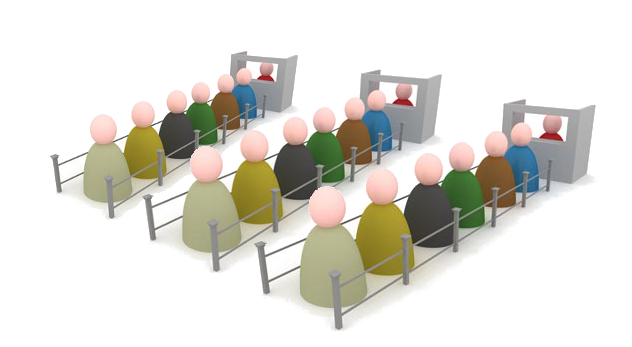
\includegraphics[scale=0.20]{img/queues.png}
  \end{center}
  \caption{Tasks queues...}
\end{figure}



\chapter{Technical background on the \textsc{Linux} kernel}

The \textsc{Linux} CPU-hotplug subsystem has been added to the kernel since
2.6.14 and has since been back-ported to branches 2.4.x and 2.2.x. Such
advanced features were needed for NUMA architectures, paravirtualized systems
or high available servers,... A more novel use of CPU-hotplug support is its
use today in suspend resume for SMP.

\paragraph{}
We'll go a step further that what it's been designed for and will use it
dynamically during system execution. Please note that what follows is more a
technical overview of the implementation of the hotplug subsystem: you don't
really need to read it to understand how the RM is working but when we started
working on it, we'd have liked to have something like this to lead off. Anyway,
as \textsc{Linux} is open source, a good look at the code \cite{vanilla} would
certainly give you much more details with less mistakes, so fell free to skip
this chapter. Please, note that explanations which follow are speacking about a
2.6.21 Linux kernel, internals structures of the scheduler have changed a lot
in 2.6.24 with the O(1) scheduler developped by Ingo Molnar.

\section{A word on the \textsc{Linux} scheduler}

You're still reading, good! Let's jump to the low levels understandings of the
scheduler. To paraphrase the introduction, the \textsc{Linux} scheduler could
be seen as a supermarket manager, the main difference is that it manages CPUs
and tasks: it is responsible for electing a certain task to run on a certain
CPU. To keep track of those tasks between different CPUs, it uses a run-queue
structure which is statically defined per CPU. This structure, extracted from
\tt{kernel/sched.c}, is shown in Listing \ref{rq}.

\paragraph{}
As we can see, the scheduler keeps two priority arrays per run-queue,
\tt{rq->active} and \tt{rq->expired} arrays, containing respectively the tasks
that still have a time-slice, and tasks that have used their time-slice. The
scheduler will elect the task which has the biggest priority in the
\tt{rq->active} array, and let it run until its time-slice finishes : it then
moves the task from the \tt{rq->active} array to the \tt{rq->expired}
array. When the \tt{rq->active} array is empty, the scheduler switches the
\tt{rq->active} and \tt{rq->expired} pointers and keeps the same logic. If
there are no tasks at all, the CPU will execute the idle thread which executes
\tt{cpu\_idle()} (\tt{cpu\_idle()} is architecture dependent, see Listing
\ref{idle}). For a non-SMP system, the explanation stops here as tasks cannot
move from one run-queue to another.

\lstset { language=C, numbers=none, numberstyle=\tiny, tabsize=8, basicstyle = \tiny }

\begin{lstlisting}[float,caption=The runqueue structure{{,}} \tt{kernel/sched.c},label=rq]
  struct rq {
        spinlock_t lock;

        unsigned long nr_running;
        unsigned long raw_weighted_load;
        unsigned long cpu_load[3];
        unsigned long long nr_switches;

        unsigned long nr_uninterruptible;

        unsigned long expired_timestamp;
        unsigned long long most_recent_timestamp;
        struct task_struct *curr, *idle;
        unsigned long next_balance;
        struct mm_struct *prev_mm;
        struct prio_array *active, *expired, arrays[2];
        int best_expired_prio;
        atomic_t nr_iowait;

        struct sched_domain *sd;

        int active_balance;
        int push_cpu;
        int cpu;

        struct task_struct *migration_thread;
        struct list_head migration_queue;

        struct lock_class_key rq_lock_key;

        ...

  };
\end{lstlisting}

\paragraph{}
However, we're interested in SMP so a task may move from one CPU to another:
here are the only 3 ways for this to happen (besides a call to \tt{
  cpu\_down(), see Listing \ref{cpudown}}):
\begin{itemize}
  \item A CPU is going to be idle (i.e. \tt{rq->active} and \tt{
    rq->expired} are empty), but first it calls \tt{idle\_balance()} to
    check if there's another CPU busy with more than one running task
    (i.e. \tt{rq->nr\_running > 1}). If this is the case, it pulls
    a task from this busy CPU and runs it instead of going idle.
  \item The CPU affinity of a certain task has been changed, and this task was
    running on a CPU that is not allowed anymore (see the \tt{taskset}
    utility for CPU affinity in user-land). The \tt{set\_cpus\_allowed()}
    in \tt{kernel/sched.c} is called and will wake up the migration thread
    to do the actual migration of tasks.
  \item The \tt{rq->next\_balance} is a sort of deadline: it is checked at each
    timer interrupt and if it's been exceeded, a \tt{ SCHED\_SOFTIRQ} is
    raised, which will trigger the \tt{ run\_rebalance\_domains()}
    function. This function checks if the load is fairly balanced between CPU
    of the same domain, and if not will set the flag \tt{rq->active\_balance}
    and wake up the migration thread. If CPU are well balanced, it resets
    \tt{rq->next\_balance} to a value in the future and returns.
\end{itemize}

You may have noticed that this is the first time the migration thread is
mentioned. This thread is CPU bounded, there is one and only one per CPU, and
it has a very high priority. Its job, as its name indicates, is to migrate
tasks from a busy CPU to the CPU it is running on (it {\em pulls} tasks from
busier CPUs than the one it's running on).

\paragraph{}
Now that we have a global view on how the scheduler manages tasks internally,
let's see the CPU hotplug internals.

\section{\textsc{Linux} CPU hotplug internals}

The CPU hotplug subsystem is not only a way to support a CPU hotplug, but it
also supports the {\em hotunplugging} of a CPU. As it may sounds more
complicated, we'll begin with it, making the hotplug a fancy task when we'll be
at it.

\subsection{Death of a CPU}

Internally, it all begins with a call to \tt{cpu\_down()}, which is triggered
when the admin writes a \tt{0} in
\tt{/sys/devices/system/cpu/cpuX/online}. Please note that this file is only
present if \tt{CONFIG\_HOTPLUG\_CPU} has been compiled in the kernel.

The best way to understand what's happening is to look at \tt{kernel/cpu.c}, you can see a
lighter version in Listing \ref{cpudown}.

\begin{lstlisting}[caption=\tt{\_cpu\_down()}{{,}} \tt{kernel/cpu.c},label=cpudown]
static int _cpu_down(unsigned int cpu)
{
        ...

        /* Tell everyone a CPU is going to die */
	err = raw_notifier_call_chain(&cpu_chain,
                                      CPU_DOWN_PREPARE,
				      (void *)(long)cpu);

        ...

	/* Ensure that we are not runnable on dying cpu */
	old_allowed = current->cpus_allowed;
	tmp = CPU_MASK_ALL;
	cpu_clear(cpu, tmp);
	set_cpus_allowed(current, tmp);

	mutex_lock(&cpu_bitmask_lock);
	p = __stop_machine_run(take_cpu_down, NULL, cpu);
	mutex_unlock(&cpu_bitmask_lock);

        ...

	/* This actually kills the CPU. */
	__cpu_die(cpu);

        ...

	/* CPU is completely dead: tell everyone */
	if (raw_notifier_call_chain(&cpu_chain, CPU_DEAD,
			(void *)(long)cpu) == NOTIFY_BAD)
		BUG();

        ...
}
\end{lstlisting}

You may have noticed that Listing \ref{cpudown} shows \tt{\_cpu\_down()} code
and not \tt{cpu\_down()}, it's because the only thing \tt{ cpu\_down()} does is
to acquire the mutex \tt{cpu\_add\_remove\_lock}, call \tt{\_cpu\_down()} and
release the lock, so that only one CPU may be removed at a time.

\paragraph{}
So what the code is doing is pretty obvious: first, it notifies every
registered callbacks that a CPU is going to be down. Second, it makes sure this
code is not running on the dying cpu by a call to \tt{ set\_cpus\_allowed()}
with a bit-mask containing all CPUs but the dying one. Next, it calls
\tt{\_\_stop\_machine\_run()}, which will create a new thread running on the
dying CPU, which then will execute the \tt{ take\_cpu\_down()} (Listing
\ref{takecpudown}) function and return.

\begin{lstlisting}[caption=\tt{take\_cpu\_down()}{{,}} \tt{kernel/cpu.c},label=takecpudown]
static int take_cpu_down(void *unused)
{
	int err;

	/* Ensure this CPU doesn't handle any more interrupts. */
	err = __cpu_disable();
	if (err < 0)
		return err;

	/* Force idle task to run as soon as we yield: it should
	   immediately notice cpu is offline and die quickly. */
	sched_idle_next();
	return 0;
}
\end{lstlisting}

The thread running on the dying CPU will, concurrently to \tt{ \_cpu\_down()},
call the architecture dependent code to disable a CPU
(\tt{\_\_cpu\_disable()}), which is responsible for clearing the the dying CPU
from the \tt{online\_map} and reroute interrupts handled by this CPU. The
\tt{online\_map} is a global bit-mask used by the scheduler to know which CPUs
are online. When this is done, the CPU will execute \tt{ cpu\_idle()}, waiting
for its actual death (unplug, or in our case, stopping its clock). Let's go
back to Listing \ref{cpudown}.

\paragraph{}
So while the dying CPU is converging to \tt{cpu\_idle()}, \tt{ \_cpu\_down()}
is still running on another CPU. The next thing it does is calling the
architecture dependent function \tt{\_\_cpu\_die()} which should wait for the
dying CPU to be idle. This is easily implemented with a flag defined per CPU,
which will be set by \tt{cpu\_idle()} when it notices that it is running on an
offline CPU (i.e. the CPU is not present in the \tt{online\_map} bit-field),
the code is shown in Listing \ref{idle}.

Finally, when \tt{\_\_cpu\_die()} returns, we are sure that the CPU is not
present anymore in the \tt{online\_map}, it doesn't treat anymore
interrupts and it is looping in \tt{cpu\_idle()}, in other terms it is
dead. The final step of \tt{\_cpu\_down()} is to tell everyone the CPU is
actually dead, which will trigger \tt{migration\_call()}, shown in Listing
\ref{migration}.

\begin{lstlisting}[caption=\tt{migration\_call()}{{,}} \tt{kernel/sched.c},label=migration]
migration_call(struct notifier_block *nfb, unsigned long action, void *hcpu)
{

        switch (action) {

        ...

	case CPU_DEAD:
		migrate_live_tasks(cpu);

		rq = cpu_rq(cpu);
		kthread_stop(rq->migration_thread);
		rq->migration_thread = NULL;

		/* Idle task back to normal  */
		rq = task_rq_lock(rq->idle, &flags);
		deactivate_task(rq->idle, rq);
		rq->idle->static_prio = MAX_PRIO;

		__setscheduler(rq->idle, SCHED_NORMAL, 0);

		migrate_dead_tasks(cpu);
		task_rq_unlock(rq, &flags);
		migrate_nr_uninterruptible(rq);
		BUG_ON(rq->nr_running != 0);

                ...

                break;

        ...

        }

        return NOTIFY_OK;

}
\end{lstlisting}

\paragraph{}
Migrate all tasks which were running on the dead CPU to another CPU is the last
thing to do before returning from \tt{\_cpu\_down()}, and this a job for
\tt{migration\_call()} which will find a CPU for those orphans tasks thanks to
\tt{migrate\_live\_tasks()}. The migration thread is bounded to the CPU so it's
not possible to run it on another CPU, and the last thing to do now is to kill
it, and this what is done in the code.

Well done! The CPU is not logically present in the system anymore, the tasks
which were running on it have moved to another CPU and no more interrupts are
treated by this CPU, so we can now remove safely the CPU. It is now time to
know what's happening on a hotplug.

\subsection{Birth of a CPU}

\paragraph{}
I'll try to explain the hotplug of a CPU in our context, that is, not stricly
spoken a hotplug, but more a reignition. Remember that we never actually
removed physically the CPU from the system, it is not present logically anymore
(the scheduler never elects a task to run on it), and the CPU doesn't consume
much energy as it is not fed with a clock, but still it is supplied a voltage,
and its internal state is preserved (see next section for a more detailed
explanation).

\paragraph{}
So when we look back at where the CPU was before stopping its clock, the CPU
shouldn't have moved from there. If we start back its clock, it'd still be in
{\tt cpu\_idle()}, busy looping untill {\tt need\_resched()} returns true, which
would never occur as that particular CPU shouldn't be present in the {\tt
  cpu\_online\_map}. So, what a hotplug is in our context is: first, starting
back the CPU clock, which will make it run {\tt cpu\_idle()}, and then adding it
to the {\tt online\_map}. As the CPU is now logically present in the system, the
scheduler may give it some task to run, and {\tt need\_resched()} whould return
{\tt true} : a CPU has just rebirth!

\paragraph{}
In a context where the CPU is actually physically plugged in, it'd fetch code
at a default address, which is generally the bootloader code. The bootloader
should identify that it is booting on a CPU that is not the master one and then
jump on the entry point of Linux. From there, the kernel would initializes
static datas that belongs to this newly added CPU, and will finally end in {\tt
  cpu\_idle()}. Now, the CPU has been physically hotplugged in, but the
scheduler still doesn't know about it as it's not in the {\tt online\_map}. For
the system to be aware of that CPU, the admin should just write a 1 in
\tt{/sys/devices/system/cpu/cpuX/online}.

\section{The clock manager support}

The CM is an IP designed by Scaleochip, it permits to stop a CPU clock and
start it back later. It's important to understand that stopping a CPU clock
freezes the corresponding CPU exactly where it is, maintaining its internal
state (cache, registers, etc\ldots), so enabling back its clock later will make
that CPU continue right where it was, with a probably corrupted cache. Knowing
that, it's important to invalidate the CPU cache right after starting back its
clock because there is great chance that the cache is corrupted.

As we've seen earlier, a dying CPU will execute \tt{cpu\_idle()} until it is
waken up, so when we'll stop its clock, we have to make sure it has reached
\tt{cpu\_idle()}. This is implemented by adding a flag defined per cpu, named
\tt{cpu\_dead}, which will be set in \tt{cpu\_idle()} when it notices it's
offline (see code in Listing \ref{idle}). Please note that this code has been
added for the sparc architecture in the scope of the SCALOPES project and has
not been merged with the vanilla kernel.

\begin{lstlisting}[caption=\tt{cpu\_idle()}{{,}} \tt{arch/sparc/process.c},label=idle]
void cpu_idle(void)
{

        ...

	while(1) {
		while (!need_resched()) {
			if (!cpu_dead(cpu) && !cpu_online(cpu))
                                /* Acked in __cpu_die */
				cpu_dead(cpu) = 1;

			cpu_relax();
		}
		if (cpu_dead(cpu) && cpu_online(cpu)) {

			/* Cleaning cache after rebirth */
			local_flush_tlb_all();
			local_flush_cache_all();

			/* We're not dead anymore */
			cpu_dead(cpu) = 0;
		}

                ...

		schedule();

                ...

	}
}
\end{lstlisting}

Observe that the cache and TLB (Table Look-aside Buffer) are invalidated when
we detect that this is a rebirth of the CPU. There's also a comment saying that
the flag is acked in \tt{\_\_cpu\_die()}, which is shown in Listing
\ref{die}. Remember that \tt{cpu\_die()} is architecture dependent, and it was
not implemented for sparc (i.e. this code is, again, not part of the vanilla
kernel).

\begin{lstlisting}[caption=\tt{\_\_cpu\_die()}{{,}} \tt{arch/sparc/smp.c},label=die]
void __cpu_die(unsigned int cpu)
{
	unsigned int	i = 0;

	/* Check that the cpu is dead */
	for (i = 0; i < 15; ++i) {
		if (cpu_dead(cpu)) { /* Acking the flag from cpu_idle() */

			/* Shut down the clock */
			__stop_cpu_clock(cpu);

			printk(KERN_INFO "CPU %d is dead.\n", cpu);
			return;
		}
		msleep(100);
	}
 	printk(KERN_ERR "CPU %u didn't die...\n", cpu);
}
\end{lstlisting}

As you can see, the code is pretty simple. It waits in a busy loop for the
dying CPU to go through \tt{cpu\_idle()}, when this is the case we shut its
clock thanks to the CM from Scaleochip. The code involved to actually ask the
CM to shut the CPU clock is just a bit to set in a particular register, so
there's no much interest in copying it here.

\paragraph{}
The last thing that misses here is the code of \tt{\_\_cpu\_disable()}, which
is also architecture dependent and, again, was not present for the sparc
architecture. Our implementation is very simple and just clear the dying CPU
from the \tt{online\_map} global. So the hotplug feature is now implemented
for our platform and is taking into account the CM, now it is time to do that
task dynamically, this is the role of the RM.

\chapter{Implementation of the RM}

Now that you're an expert on the \textsc{Linux} hotplug subsystem, it is time
to jump on the implementation of the RM. This chapter will describe what
heuristics were chosen to determine the optimal number of CPUs and the
parameters that deal with the RM behaviour.

\section{Self-balance the number of CPUs}

Let's keep with the supermarket analogy and go a bit deeper in the
reflexion. As we already make out, the best scenario would be to have one
cashier and only one by client, meaning that each time a cashier is idling, we
tell him to close its cash (i.e. he's not being paid anymore for its work). It
also means that if all cashiers are busy and a client comes up, we have to open
a new cash right away. There are a couple problems with that approach.

\paragraph{}
First, the obvious one: when a client arrives with only one article, he forces
us to open a cashier just for him and to close it as soon as he's paid. If we
go back on the RM, it means we've started back a CPU for a {\em relatively}
short task, and that we've stopped it right after. If the word {\em relatively}
is emphased, it's because it really much depends on how reactive we want to be
with our tasks, and thus this should be configurable for a particular
application.

\paragraph{}
The second problem, much less obvious at first, depends more on the number of
clients waiting behind a cash. Let's make a complete example : we have four
cashiers opened and, at checking time, all four cashiers are telling us (we are
the RM in this example) that they've been working the whole time since last
check, meaning their load is approximately 100\%. If we stop the check here,
without asking the number of clients that were waiting behind the cash, it
seems a good idea to open a new cash right now because if all four cashiers
were 100\% {\it loaded}: there are certainly some clients waiting.

Now let's suppose all cashiers were working with only one client without
anybody waiting for a cash to be available, openning a new cash would be
catastrophic, because all four precedly opened cashiers would still be 100\%,
serving the same client they were serving before the check, and the new cash
wouldn't serve anybody, meaning we are paying a cashier for nothing.

With CPUs the problem is exactly the same, if a task is using a CPUs
intensively (in the \textsc{Linux} kernel, those tasks are called CPU-bounded
tasks), the CPU will certainly appears 100\% loaded, but starting a new one at
that time may not be the best solution, because if there is only one task to
run, the new CPU will be idling and we're going to stop it right after.

\paragraph{}
To sum things up, we've seen that the decision to start back a CPU should be
taken regarding two inputs : the smoothed average load of a CPU (to be more or
less sensitive to short tasks that would make the load increase dramatically in
a short period of time), and the number of tasks which were waiting for a CPU
to be available (to not start back a CPU that is going to be useless). The
action to start back a CPU could be taken when those two comparisons become
true:

\[
\left\{
\begin{array}{lrl}
smooth\_load & > & \textsc{high\_load\_limit} \\
 & & \\
\frac{nr\_running\_tasks}{nr\_cpus} & > &  1
\end{array}
\right.
\]

On the other side, the decision to stop a CPU is much easier to take as we only
have to check if by stopping a CPU, the sum of loads on each CPU could fit in
the actual number of CPU minus one if all those remaining CPUs were 100\%
loaded, that is, if:

\[ \frac{nr\_cpus * smooth\_load}{(nr\_cpus - 1) * 100} < 1 \]

is verified, then it is time to stop a CPU. You may want to know what is this
$smooth\_load$ all about, as its name tells it is a value which indicates us a
smoothed average load of the system, see next section to know how it is
calculated.

\subsection{Smoothing the average load of a CPU}

To adjust our sensitivity to tasks that take a lot of CPU time but for a short
period, we introduce a so-called $smooth\_load$, which is defined per cpu and
is updated at the same periodicity than the RM loop (the periodicity in Hz may
be set thanks to the \tt{/proc/rm/periodicity} file and cannot exceed
10Hz). This $smooth\_load$ is a value between 0 and 100, and it
increases/decreases proportionally to the difference between the actual value
of $smooth\_load$ and the average load of the CPU since the last check. In the
source code, the value S we add to $smooth\_load$ is defined like that :

\[ S = \frac{\Delta_{load}}{P} \]

Where $P$ is a coefficient set by the administrator for a particular
application and $\Delta_{load}$ is the difference between the $average\_load$:
\[average\_load = \sum_{i=1}^{nr\_cpus} cpu\_load_i\]
and the last $smooth\_load$ calculated. The bigger $P$ is, the less sensitive
the RM will be to variations. As the cost of a CPU kill is not very important
on our platform, $P = 4$ gave us good response times while still preventing
very short task from starting back a CPU for nothing. This parameter may be
adjusted thanks to the (\tt{/proc/rm/smooth\_coeff}) file.

\subsection{Why not predicting the future ?}

The RM is implemented by making a thread which will, at a certain periodicity,
look at the system load at a whole and take a decision based on that. One could
say that we are always one step behind by acting on what happened since last
check, and he'd be right. That's a fact, we're taking decision based on an
smoothed average load and a number of tasks that {\em were} running just before
the check. One could also argue that, for starting back a CPU, at least, we
could have place a portion of code in the task creation area; that code could
check just before creating and running the task if the system is heavely
loaded, and decide to start back a CPU immediatly and run the new task on it.

In fact, that's not necessarily a good thing: the problem if we would have done
that is the same as being to sensitive on very short tasks, we're taking the
chance that the task is very very short and that we started back a CPU for
almost nothing. For example, somebody that is using intensively its terminal,
running very short commands like \tt{ls}, \tt{sleep}, \tt{grep} could suffer
from big latency if each time he runs a command, a CPU is started back, and
stopped immedialty after the command termination. We have no way of knowing how
much time a program would run, so taking the decision before observing the
behaviour of the task is risky.

On a supermarket, the question would be easily solved because with the size of
the cart, we could estimate the time a client would take on the cashier. On the
\textsc{Linux} kernel side, the extension of that idea would be to collect some
statistics on the execution time of programs, that would implie a lot of
modifications which we don't really need in the SCALOPES scope: for now on, the
behaviour of the RM is quite satisfactory for our use. Further, the
introduction of those stats would certainly slow down the \textsc{Linux}
kernel.

\section{Introducing a performance loss parameter}

Up to now, we've tried to cut down the current consumption without altering the
performance of the machine (considering that the birth and death of a CPU are
negligible). What the RM also permits is to set a performance loss parameter,
which is defined as the maximum performance lost allowed. It is configurable
through the \tt{/proc/rm/perf\_loss} file. If we go back to the comparisons
exposed in the last section, we were always comparing to $1$, which is now
replaced by
\[1 * \left(\frac{100}{perf\_loss}\right)\]

Let's see the effect of this parameter on the decision to start a CPU for a
lost of performance equal to 50. As we've seen earlier, to start back a CPU, we
have to be higher than a certain hard-coded limit called
\textsc{high\_load\_limit}, this comparison doesn't change, and the average
number of tasks running on one CPU should be superior than $1 * \frac{100}{50}
= 2$, not $1$. We've multiplied by 2 the number of running tasks allowed by CPU
when the load is more than the limit fixed, which should decrease the
performances of those 2 tasks by 2 if the scheduling algorithm fairly shares
the CPU time between those two. By reflection, the decision to stop a CPU will
be taken when $nr\_cpus * smooth\_load$ is two times more than $(nr\_cpus - 1)
* 100$.

\chapter{Measures of performance and power consumption}

\chapter{Conclusion}

\bibliographystyle{plain}
\bibliography{rm_scaleo.bib}

\end{document}

